\documentclass[aspectratio=169, 10pt]{beamer}

% ==============================================================================
% THEME & COLOR CONFIGURATION (BEAMER MADRID)
% ==============================================================================
\usetheme{Madrid}
\useinnertheme{rectangles}

% Bảng màu thương hiệu PetCare Pro (Hài hòa giữa Navy HCMUS và Teal hiện đại)
\definecolor{PetcarePrimary}{RGB}{23, 59, 114}    % #173B72 Deep Navy Blue (HCMUS)
\definecolor{PetcareSecondary}{RGB}{13, 148, 136} % #0D9488 Vibrant Teal
\definecolor{PetcareAccent}{RGB}{217, 119, 6}    % #D97706 Warm Amber/Orange
\definecolor{PetcareAlert}{RGB}{220, 38, 38}     % #DC2626 Medical Alert Red
\definecolor{PetcareDark}{RGB}{30, 41, 59}       % #1E293B Slate 800
\definecolor{PetcareLight}{RGB}{248, 250, 252}   % #F8FAFC Slate 50
\definecolor{PetcareCardBg}{RGB}{241, 245, 249}  % #F1F5F9 Slate 100
\definecolor{PetcareSuccess}{RGB}{22, 163, 74}   % #16A34A Success Green

% Thiết lập phối màu Beamer Madrid
\setbeamercolor{structure}{fg=PetcarePrimary}
\setbeamercolor{palette primary}{bg=PetcarePrimary,fg=white}
\setbeamercolor{palette secondary}{bg=PetcareSecondary,fg=white}
\setbeamercolor{palette tertiary}{bg=PetcareDark,fg=white}
\setbeamercolor{palette quaternary}{bg=PetcarePrimary,fg=white}

\setbeamercolor{titlelike}{parent=palette primary,fg=PetcarePrimary}
\setbeamercolor{frametitle}{bg=PetcarePrimary!8,fg=PetcarePrimary}
\setbeamercolor{frametitle right}{bg=PetcareSecondary!10}

% Khối hộp Beamer (Blocks)
\setbeamercolor{block title}{bg=PetcarePrimary,fg=white}
\setbeamercolor{block body}{bg=PetcareCardBg,fg=PetcareDark}
\setbeamercolor{block title example}{bg=PetcareSecondary,fg=white}
\setbeamercolor{block body example}{bg=PetcareCardBg,fg=PetcareDark}
\setbeamercolor{block title alerted}{bg=PetcareAlert,fg=white}
\setbeamercolor{block body alerted}{bg=PetcareAlert!8,fg=PetcareDark}

% Loại bỏ thanh điều hướng mặc định ở góc dưới để giữ giao diện tối giản
\setbeamertemplate{navigation symbols}{}

% Tùy biến Footline Madrid: Tác giả | Tên đề tài rút gọn | Ngày & Số trang
\setbeamertemplate{footline}{%
  \leavevmode%
  \hbox{%
  \begin{beamercolorbox}[wd=.30\paperwidth,ht=2.25ex,dp=1ex,center]{author in head/foot}%
    \usebeamerfont{author in head/foot}\textbf{Nhóm 10} (L.N.Q. Bảo, N.Q. Bảo, N.T. Tín)
  \end{beamercolorbox}%
  \begin{beamercolorbox}[wd=.45\paperwidth,ht=2.25ex,dp=1ex,center]{title in head/foot}%
    \usebeamerfont{title in head/foot}\textbf{Hệ thống hỗ trợ chăm sóc thú cưng}
  \end{beamercolorbox}%
  \begin{beamercolorbox}[wd=.25\paperwidth,ht=2.25ex,dp=1ex,right]{date in head/foot}%
    \usebeamerfont{date in head/foot}CSC12106 \quad \insertframenumber{} / \inserttotalframenumber\hspace*{2ex}
  \end{beamercolorbox}}%
  \vskip0pt%
}

% ==============================================================================
% PACKAGES & FONT (XELATEX TIẾNG VIỆT)
% ==============================================================================
\usepackage{fontspec}
\defaultfontfeatures{Ligatures=TeX}
\setmainfont{Times New Roman}
\setsansfont{Times New Roman}

\usepackage{graphicx}
\usepackage{booktabs}
\usepackage{tabularx}
\usepackage{colortbl}
\usepackage{tikz}
\usepackage{multicol}

% ==============================================================================
% THÔNG TIN BÁO CÁO & TRANG BÌA
% ==============================================================================
\title[PetCare Pro Mobile App]{HỆ THỐNG HỖ TRỢ ĐẶT LỊCH, GỬI YÊU CẦU\texorpdfstring{\\}{ }VÀ THEO DÕI QUÁ TRÌNH CHĂM SÓC THÚ CƯNG}
\subtitle{Báo cáo Đồ án môn học Tương tác Người -- Máy (CSC12106)}

\author[Nhóm 10]{%
  \textbf{Sinh viên thực hiện:}\\[1mm]
  23127327 -- Lưu Ngô Quốc Bảo\\
  23127328 -- Nguyễn Quốc Bảo\\
  23127498 -- Nguyễn Trọng Tín%
}

\institute[HCMUS]{%
  \textbf{Giảng viên hướng dẫn:} Lê Thị Nhàn, Lương Vĩ Minh\\[1mm]
  \textit{Khoa Công nghệ Thông tin -- Trường Đại học Khoa học Tự nhiên, ĐHQG-HCM}
}

\date{Tháng 09 năm 2026}

% ==============================================================================
% BẮT ĐẦU NỘI DUNG SLIDE
% ==============================================================================
\begin{document}

% Slide 1: Trang bìa
% Slide 1: Trang tiêu đề
{
\setbeamertemplate{footline}{} % Ẩn footline ở trang bìa
\begin{frame}[plain]
  \begin{tikzpicture}[remember picture, overlay]
    % Dải banner màu xanh thương hiệu ở đầu trang
    \fill[PetcarePrimary] (current page.north west) rectangle ([yshift=-1.2cm]current page.north east);
    % Logo trường HCMUS góc trên bên phải
    \node[anchor=north east, inner sep=6pt] at (current page.north east) {
      
\includegraphics[height=1.0cm, keepaspectratio]{img/hcmus-logo.png}
    };
    % Tên trường góc trên bên trái
    \node[anchor=north west, inner sep=10pt] at (current page.north west) {
      \small \bfseries \color{white} TRƯỜNG ĐẠI HỌC KHOA HỌC TỰ NHIÊN -- ĐHQG-HCM
    };
  \end{tikzpicture}

  \vspace{0.6cm}

  \begin{center}
    {\scriptsize \color{PetcareSecondary}\textbf{ĐỒ ÁN MÔN HỌC: TƯƠNG TÁC NGƯỜI -- MÁY (CSC12106)}}\\[2mm]
    {\large \bfseries \color{PetcarePrimary} HỆ THỐNG HỖ TRỢ ĐẶT LỊCH, GỬI YÊU CẦU\\VÀ THEO DÕI QUÁ TRÌNH CHĂM SÓC THÚ CƯNG}\\[1.5mm]
    {\footnotesize \color{PetcareDark}\textit{Giải pháp tương tác di động lấy chủ nuôi thú cưng bận rộn làm trung tâm (UCD)}}
  \end{center}

  \vspace{0.2cm}

  \begin{columns}[c]
    \begin{column}{0.50\textwidth}
      \begin{block}{\footnotesize \textbf{Sinh viên thực hiện (Nhóm 10)}}
        \scriptsize
        \textbf{23127327} -- Lưu Ngô Quốc Bảo\\
        \textbf{23127328} -- Nguyễn Quốc Bảo\\
        \textbf{23127498} -- Nguyễn Trọng Tín
      \end{block}
    \end{column}
    \begin{column}{0.46\textwidth}
      \begin{block}{\footnotesize \textbf{Giảng viên hướng dẫn}}
        \scriptsize
        \textbf{Lê Thị Nhàn}\\
        \textbf{Lương Vĩ Minh}\\[1.5mm]
        \textit{Khoa Công nghệ Thông tin}
      \end{block}
    \end{column}
  \end{columns}

  \vspace{0.2cm}
  \begin{center}
    {\tiny \color{gray} Thành phố Hồ Chí Minh, Tháng 09 năm 2026}
  \end{center}
\end{frame}
}


% Slide 2: Executive Hook - Bối cảnh & 4 Điểm đau
% Slide 2: Executive Hook - Bối cảnh & 4 Điểm đau cốt lõi
\begin{frame}{Bối Cảnh Đề Tài \& Phát Biểu Bài Toán}
  \framesubtitle{\color{PetcareSecondary}\textbf{Nghịch lý thời gian: Khi chủ nuôi bận rộn đối mặt với quy trình thủ công phân mảnh}}

  \begin{columns}[T]
    % Cột trái: 4 Điểm đau cốt lõi (Bullet súc tích)
    \begin{column}{0.58\textwidth}
      \begin{itemize}
        \setlength\itemsep{0.4mm}
        \footnotesize
        \item \textbf{Khó khăn đặt lịch \& chờ đợi:} Phải gọi điện/nhắn tin hỏi lịch, chờ phản hồi lâu, dễ bị trùng lịch hoặc lỡ khung giờ đẹp.
        \item \textbf{Thất lạc dặn dò y tế \& dị ứng:} Tiền sử dị ứng xà phòng/thuốc dễ bị nhân viên bỏ sót khi đổi ca trực, tiềm ẩn nguy cơ viêm da.
        \item \textbf{Mù mờ tiến độ thời gian thực:} Khoảng trống thông tin 2--3 tiếng đẩy chủ nuôi vào tâm lý bất an nhưng ngại gọi điện làm phiền.
        \item \textbf{Mất dấu lịch sử \& hóa đơn:} Không có nhật ký chăm sóc tập trung, khó tra cứu loại dầu tắm đã dùng và quản lý chi tiêu.
      \end{itemize}
    \end{column}

    % Cột phải: 3 Thẻ số liệu cảnh báo (Metric Alert Callouts)
    \begin{column}{0.38\textwidth}
      \begin{alertblock}{\centering \scriptsize \textbf{Thời gian chờ xác nhận}}
        \centering \vspace{0.2mm}
        {\large \textbf{15 -- 120 phút}}\\[0.2mm]
        {\tiny \color{PetcareDark}Chờ phản hồi qua tin nhắn/cuộc gọi}
      \end{alertblock}

      \vspace{-1.5mm}
      \begin{alertblock}{\centering \scriptsize \textbf{Xác suất quên dặn dò}}
        \centering \vspace{0.2mm}
        {\large \textbf{$>$ 80\% nguy cơ}}\\[0.2mm]
        {\tiny \color{PetcareDark}Khi chuyển giao ca trực hoặc ghi sổ tay}
      \end{alertblock}

      \vspace{-1.5mm}
      \begin{alertblock}{\centering \scriptsize \textbf{Điểm mù tiến độ (Black-box)}}
        \centering \vspace{0.2mm}
        {\large \textbf{2 -- 3 tiếng}}\\[0.2mm]
        {\tiny \color{PetcareDark}Mù mờ thông tin trạng thái thú cưng}
      \end{alertblock}
    \end{column}
  \end{columns}

  \vspace{0.2mm}
  \begin{block}{\scriptsize \textbf{Mục tiêu cốt lõi}}
    \tiny \textbf{Giải pháp tương tác di động Mobile-first}: Đặt lịch xác nhận tức thì $\bullet$ Cảnh báo y tế tự động $\bullet$ Live Tracking 4 mốc $\bullet$ Nhật ký cá nhân hóa.
  \end{block}
\end{frame}


% Slide 3: Nghiên cứu người dùng & Bằng chứng thực địa
% Slide 3: Nghiên cứu người dùng & Bằng chứng thực địa
\begin{frame}{Nghiên Cứu Người Dùng \& Phát Hiện Then Chốt}
  \framesubtitle{\color{PetcareSecondary}\textbf{Tiếng nói từ thực địa: Dữ liệu phỏng vấn sâu và 4 phát hiện bước ngoặt}}

  \begin{columns}[T]
    % Cột trái: 4 Phát hiện thực nghiệm (Key Findings)
    \begin{column}{0.56\textwidth}
      \begin{itemize}
        \setlength\itemsep{1.2mm}
        \footnotesize
        \item \textbf{100\% Gặp sự cố đặt lịch:} Chờ phản hồi lâu (15p--2h); nhiều trường hợp bị người khác đặt mất chỗ trong lúc chờ nhắn tin.
        \item \textbf{83.3\% Bất an về dị ứng da:} Chủ nuôi có thú cưng da nhạy cảm luôn sợ tiệm dùng nhầm sữa tắm kích ứng khi đổi ca trực.
        \item \textbf{90\% Lo âu kéo dài:} Bồn chồn trong suốt 2--3 tiếng gửi bé, nhưng $>$ 70\% ngại gọi điện chen ngang công việc của tiệm.
        \item \textbf{100\% Thiếu kho lưu trữ:} Thông tin hóa đơn, ngày tiêm phòng và loại sữa tắm trị liệu bị trôi dạt hoàn toàn trong tin nhắn cũ.
      \end{itemize}
    \end{column}

    % Cột phải: Phương pháp nghiên cứu & Trích dẫn thực tế (User Quote)
    \begin{column}{0.40\textwidth}
      \begin{block}{\centering \scriptsize \textbf{Phương pháp nghiên cứu chuẩn HCI}}
        \scriptsize
        $\bullet$ \textbf{Phỏng vấn sâu:} 6 chủ nuôi tại TP.HCM.\\
        $\bullet$ \textbf{Khảo sát trực tuyến:} Thói quen \& rào cản.
      \end{block}

      \vspace{-1mm}
      \begin{exampleblock}{\scriptsize \textbf{Tiếng nói từ người dùng thực tế}}
        \tiny \textit{``Mỗi lần gửi cún đi spa là mình phải dặn đi dặn lại chuyện bé dị ứng xà phòng có mùi nồng, nhưng tiệm đổi ca vẫn thỉnh thoảng quên làm bé ngứa gãi đỏ cả người...''}\\[1mm]
        \hfill \textbf{--- Chị Lan (28t, Chuyên viên phân tích, Q.1)}
      \end{exampleblock}
    \end{column}
  \end{columns}

  \vspace{1.5mm}
  % Dải số liệu nổi bật chân trang
  \begin{columns}[c]
    \begin{column}{0.24\textwidth}
      \begin{block}{\centering \tiny \textbf{Trì trệ đặt lịch}}
        \centering \footnotesize \textbf{\color{PetcareAlert}100\%} \tiny gặp sự cố
      \end{block}
    \end{column}
    \begin{column}{0.24\textwidth}
      \begin{block}{\centering \tiny \textbf{Nỗi lo dị ứng da}}
        \centering \footnotesize \textbf{\color{PetcareAlert}83.3\%} \tiny lo lắng
      \end{block}
    \end{column}
    \begin{column}{0.24\textwidth}
      \begin{block}{\centering \tiny \textbf{Bất an tiến độ}}
        \centering \footnotesize \textbf{\color{PetcareAlert}90.0\%} \tiny bồn chồn
      \end{block}
    \end{column}
    \begin{column}{0.24\textwidth}
      \begin{block}{\centering \tiny \textbf{Mất dấu lịch sử}}
        \centering \footnotesize \textbf{\color{PetcareAlert}100\%} \tiny không lưu trữ
      \end{block}
    \end{column}
  \end{columns}
\end{frame}


% Slide 4: Chân dung Người dùng & Bản đồ Giá trị 1-1
% Slide 4: Chân dung Người dùng & Bản đồ Giá trị Đối ứng 1-1
\begin{frame}{Chân Dung Người Dùng \& Tuyên Ngôn Giá Trị}
  \framesubtitle{\color{PetcareSecondary}\textbf{Đồng cảm sâu sắc: 2 Chân dung khách hàng \& Bản đồ Giá trị đối ứng 1--1}}

  \begin{columns}[T]
    % Cột 1: Persona 1 (Nguyễn Hoàng Lan)
    \begin{column}{0.48\textwidth}
      \begin{block}{\footnotesize \textbf{Persona 1 (Chính) -- Nguyễn Hoàng Lan (28t)}}
        \scriptsize
        \textbf{Bối cảnh:} Chuyên viên Phân tích Dữ liệu, Q.1. Nuôi cún Poodle Bơ (4.5kg, \textit{tiền sử viêm da dị ứng xà phòng}).\\[1mm]
        \textbf{Điểm đau lớn nhất:}
        \begin{itemize}
          \tiny
          \item Chờ đợi tin nhắn đặt lịch lâu trong giờ làm việc.
          \item Nơm nớp lo tiệm quên dùng sữa tắm dịu nhẹ trị liệu.
          \item Bất an không rõ cún làm đến đâu suốt 2 tiếng.
        \end{itemize}
        \textbf{Giá trị đối ứng (Value Proposition):}
        \begin{itemize}
          \tiny
          \item \textbf{Khóa giữ chỗ tức thì} trên ma trận giờ còn trống.
          \item \textbf{Tự động gắn nhãn y tế đỏ} lên phiếu QR tiếp nhận.
          \item \textbf{Live Tracking 4 mốc} kèm thông báo đẩy tự động.
        \end{itemize}
      \end{block}
    \end{column}

    % Cột 2: Persona 2 (Trần Minh Khoa)
    \begin{column}{0.48\textwidth}
      \begin{exampleblock}{\footnotesize \textbf{Persona 2 (Phụ) -- Trần Minh Khoa (21t)}}
        \scriptsize
        \textbf{Bối cảnh:} Sinh viên ĐHQG, TP. Thủ Đức. Nuôi mèo Anh lông ngắn Miu (3.8kg, \textit{tính cách rất nhút nhát, sợ tiếng ồn}).\\[1mm]
        \textbf{Điểm đau lớn nhất:}
        \begin{itemize}
          \tiny
          \item Đến tiệm mới biết đông khách, mèo bị hoảng loạn.
          \item Ám ảnh sự cố an toàn, rất ngại gọi điện thoại hỏi.
          \item Ngân sách sinh viên, sợ phát sinh chi phí phụ.
        \end{itemize}
        \textbf{Giá trị đối ứng (Value Proposition):}
        \begin{itemize}
          \tiny
          \item \textbf{Hiển thị mật độ giờ vắng} để chủ động đặt chỗ yên tĩnh.
          \item \textbf{Thông báo trạng thái hoàn tất} để đến đón bé sớm nhất.
          \item \textbf{Bảng giá minh bạch 100\%} \& lưu trữ hóa đơn chi tiết.
        \end{itemize}
      \end{exampleblock}
    \end{column}
  \end{columns}

  \vspace{1.5mm}
  \begin{center}
    \scriptsize \color{PetcarePrimary}
    \textbf{Nguyên tắc thiết kế UCD:} Xây dựng giải pháp giải quyết đồng thời bài toán \textbf{Thời gian} của người đi làm và bài toán \textbf{An toàn tâm lý} của thú cưng nhút nhát.
  \end{center}
\end{frame}


% Slide 5: Chuyển dịch quy trình: As-Is vs To-Be
% Slide 5: Chuyển dịch quy trình: As-Is vs To-Be
\begin{frame}{Đột Phá Trải Nghiệm: Chuyển Dịch Quy Trình}
  \framesubtitle{\color{PetcareSecondary}\textbf{Tái định hình quy trình: 6 bước As-Is thủ công chuyển dịch sang 6 bước To-Be số hóa}}

  \begin{table}
    \centering
    \tiny
    \renewcommand{\arraystretch}{1.25}
    \begin{tabularx}{\textwidth}{|l|X|X|c|}
      \hline
      \rowcolor{PetcarePrimary!15}
      \textbf{Bước tác vụ} & \textbf{Quy trình cũ thủ công (As-Is)} & \textbf{Hệ thống mới số hóa (To-Be)} & \textbf{Hiệu quả đột phá} \\ \hline
      \textbf{1. Đặt lịch hẹn} & Nhắn tin/gọi điện hỏi giờ; chờ đợi đối soát sổ sách 15p--2h; dễ trùng/lỡ lịch. & Chọn giờ trống trực quan trên ma trận thời gian thực; nhận mã xác nhận tức thì. & \textbf{\color{PetcareSuccess}Rút ngắn 95\%} ($<$ 40s) \\ \hline
      \textbf{2. Dặn dò dị ứng} & Nhắc miệng hoặc gõ chat rời rạc; nhân viên đổi ca dễ bỏ sót ($>$ 80\% rủi ro). & Hồ sơ tự động gắn nhãn cảnh báo đỏ y tế lên phiếu hẹn và biên bản bàn giao. & \textbf{\color{PetcareSuccess}Triệt tiêu 100\%} rủi ro \\ \hline
      \textbf{3. Bàn giao tiếp nhận} & Khách chờ tại tiệm 10--15 phút để nhân viên ghi chép tay hoặc dán post-it. & Nhân viên quét mã QR trên app của khách; ký xác nhận biên bản an toàn 2 lớp. & \textbf{\color{PetcareSuccess}Tiết kiệm 80\%} ($<$ 1 phút) \\ \hline
      \textbf{4. Theo dõi tiến độ} & Mù mờ thông tin suốt 2--3 tiếng; chủ nuôi lo âu, gọi điện chen ngang công việc. & Thanh tiến trình 4 mốc thời gian thực; tự động gửi Push Notification từng giai đoạn. & \textbf{\color{PetcareSuccess}Minh bạch 100\%} 4 mốc \\ \hline
      \textbf{5. Đón thú cưng} & Tiệm gọi điện gián đoạn công việc; chủ nuôi bị động trong việc sắp xếp đi đón. & Nhận thông báo mời đón chuẩn xác; đối soát mã QR an toàn khi trả thú cưng. & \textbf{\color{PetcareSuccess}Chủ động 100\%} thời gian \\ \hline
      \textbf{6. Nhật ký \& Lịch sử} & Hóa đơn giấy dễ mất; quên tên sữa tắm trị liệu cũ; khó theo dõi ngân sách. & Kho lưu trữ số hóa trọn đời: phác đồ sản phẩm, ảnh sức khỏe, hóa đơn \& Rebook 1 chạm. & \textbf{\color{PetcareSuccess}Tra cứu 1 chạm} \\ \hline
    \end{tabularx}
  \end{table}

  \vspace{1mm}
  \begin{block}{\centering \scriptsize \textbf{Tác động cốt lõi}}
    \centering \tiny
    Chuyển đổi từ mô hình \textbf{Thụ động -- Phân mảnh -- Mù mờ thông tin} sang mô hình \textbf{Chủ động -- Đồng bộ -- Minh bạch thời gian thực}.
  \end{block}
\end{frame}


% Slide 6: Kiến trúc thông tin & Hệ thống Wireframe 5 UI States
% Slide 6: Kiến trúc thông tin & Hệ thống Wireframe 5 UI States
\begin{frame}{Thiết Kế Tương Tác: Kiến Trúc Thông Tin \& Wireframe}
  \framesubtitle{\color{PetcareSecondary}\textbf{Cấu trúc trực quan: Kiến trúc thông tin phẳng \& Hệ thống 32 Wireframes chuẩn UX}}

  \begin{columns}[T]
    % Cột trái: Kiến trúc thông tin & 5 UI States
    \begin{column}{0.50\textwidth}
      \begin{block}{\footnotesize \textbf{Kiến trúc thông tin phẳng (Flat IA Mobile-first)}}
        \scriptsize
        Điều hướng chính qua thanh Bottom Bar cố định gồm 4 phân hệ:
        \begin{enumerate}
          \tiny
          \item \textbf{Trang chủ (Home):} Thẻ thú cưng, nhắc lịch hẹn, phím tắt.
          \item \textbf{Đặt lịch (Booking):} Chọn dịch vụ, ma trận giờ, xác nhận.
          \item \textbf{Tiến độ (Tracking):} 4 mốc thời gian, ảnh khám, gửi dặn dò.
          \item \textbf{Hồ sơ \& Lịch sử (Profile):} Cảnh báo dị ứng, hóa đơn, Rebook.
        \end{enumerate}
      \end{block}

      \vspace{-1mm}
      \begin{exampleblock}{\footnotesize \textbf{Bao phủ trọn vẹn 5 Trạng thái giao diện (UI States)}}
        \tiny
        $\bullet$ \textbf{Ideal State:} Dữ liệu đầy đủ, ma trận giờ trực quan.\\
        $\bullet$ \textbf{Loading State:} Hiệu ứng Skeleton Loading chống giật màn hình.\\
        $\bullet$ \textbf{Empty State:} Minh họa thân thiện kèm nút kêu gọi hành động (CTA).\\
        $\bullet$ \textbf{Error/Conflict State:} Báo xung đột dị ứng \& mã QR cứu hộ offline.\\
        $\bullet$ \textbf{Success State:} Chúc mừng kèm mã đặt lịch và QR tiếp nhận ngay.
      \end{exampleblock}
    \end{column}

    % Cột phải: 3 Màn hình Wireframe minh họa
    \begin{column}{0.48\textwidth}
      \centering
      \begin{columns}[c]
        \begin{column}{0.32\textwidth}
          \centering
          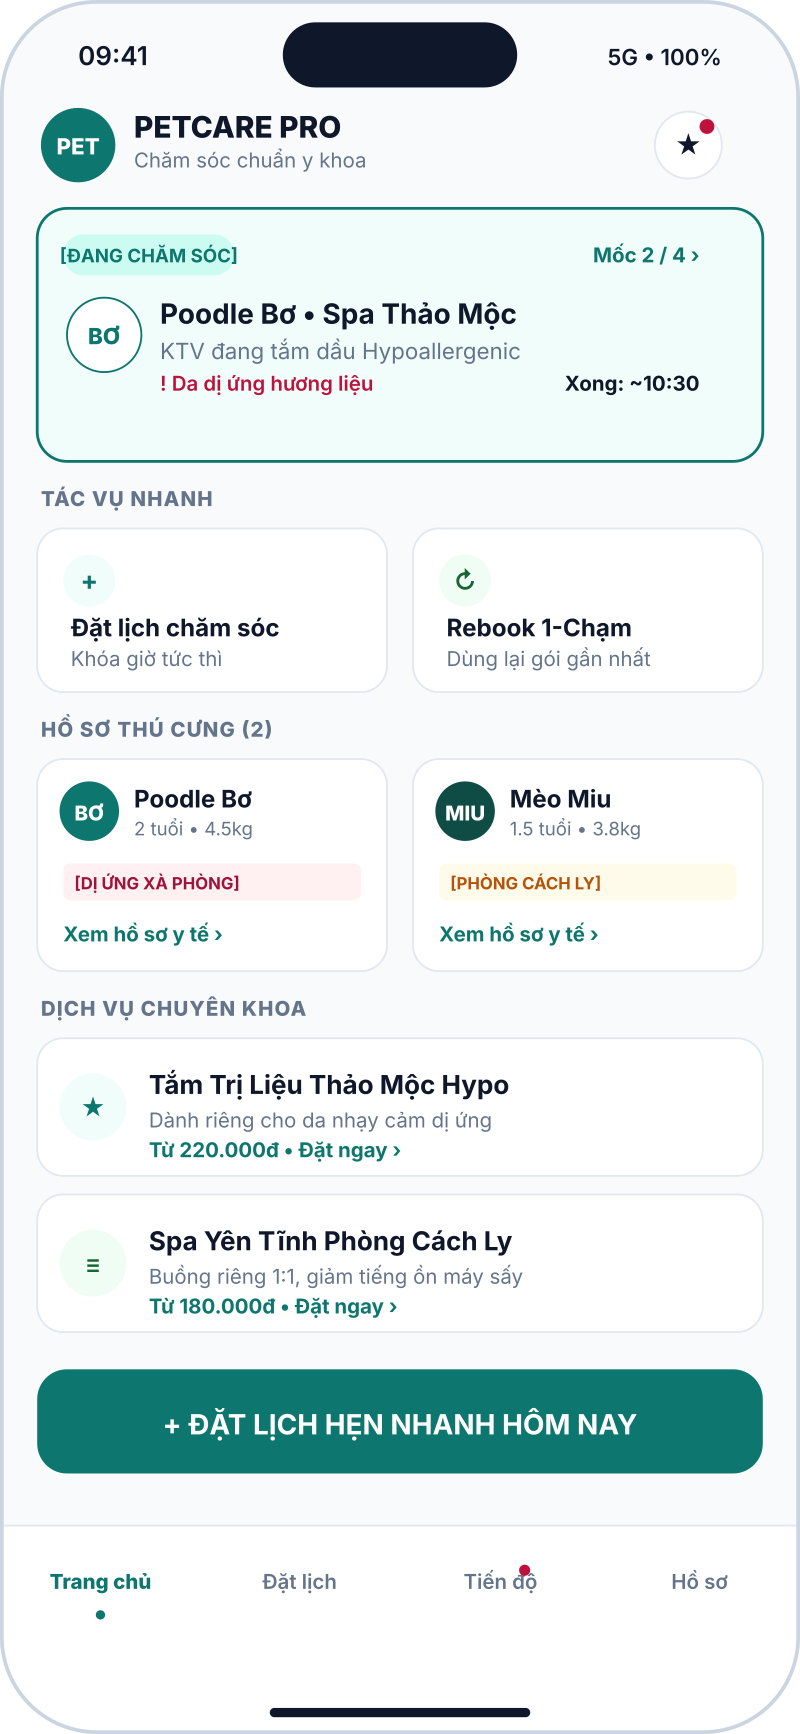
\includegraphics[height=4.4cm, keepaspectratio]{img/wf_01_home.png}\\[0.5mm]
          {\tiny \textbf{Trang chủ}}
        \end{column}
        \begin{column}{0.32\textwidth}
          \centering
          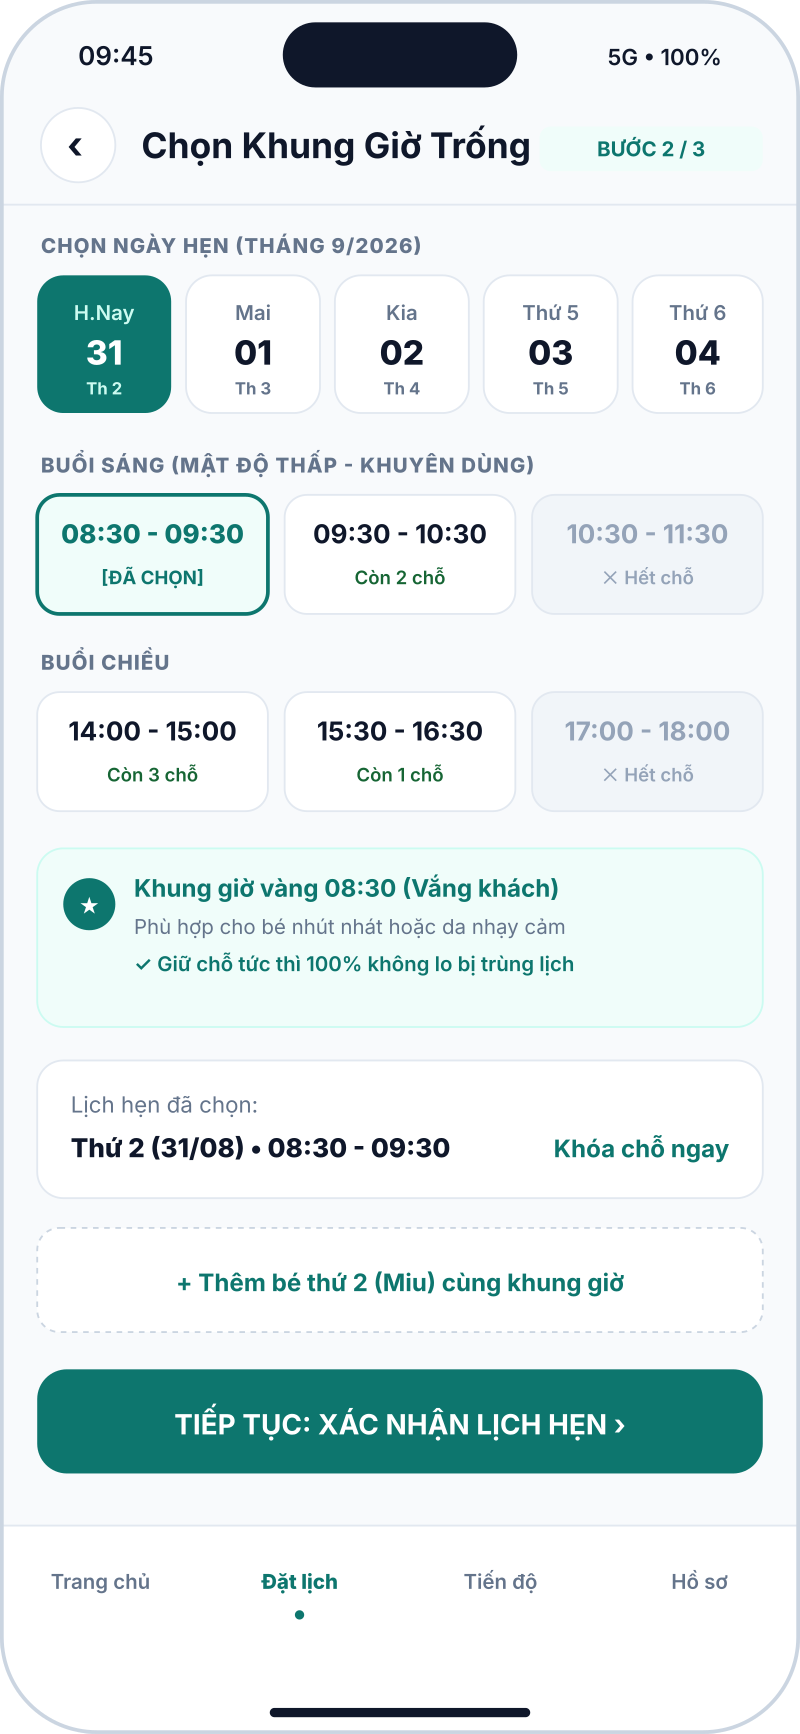
\includegraphics[height=4.4cm, keepaspectratio]{img/wf_05_timeslot.png}\\[0.5mm]
          {\tiny \textbf{Ma trận giờ}}
        \end{column}
        \begin{column}{0.32\textwidth}
          \centering
          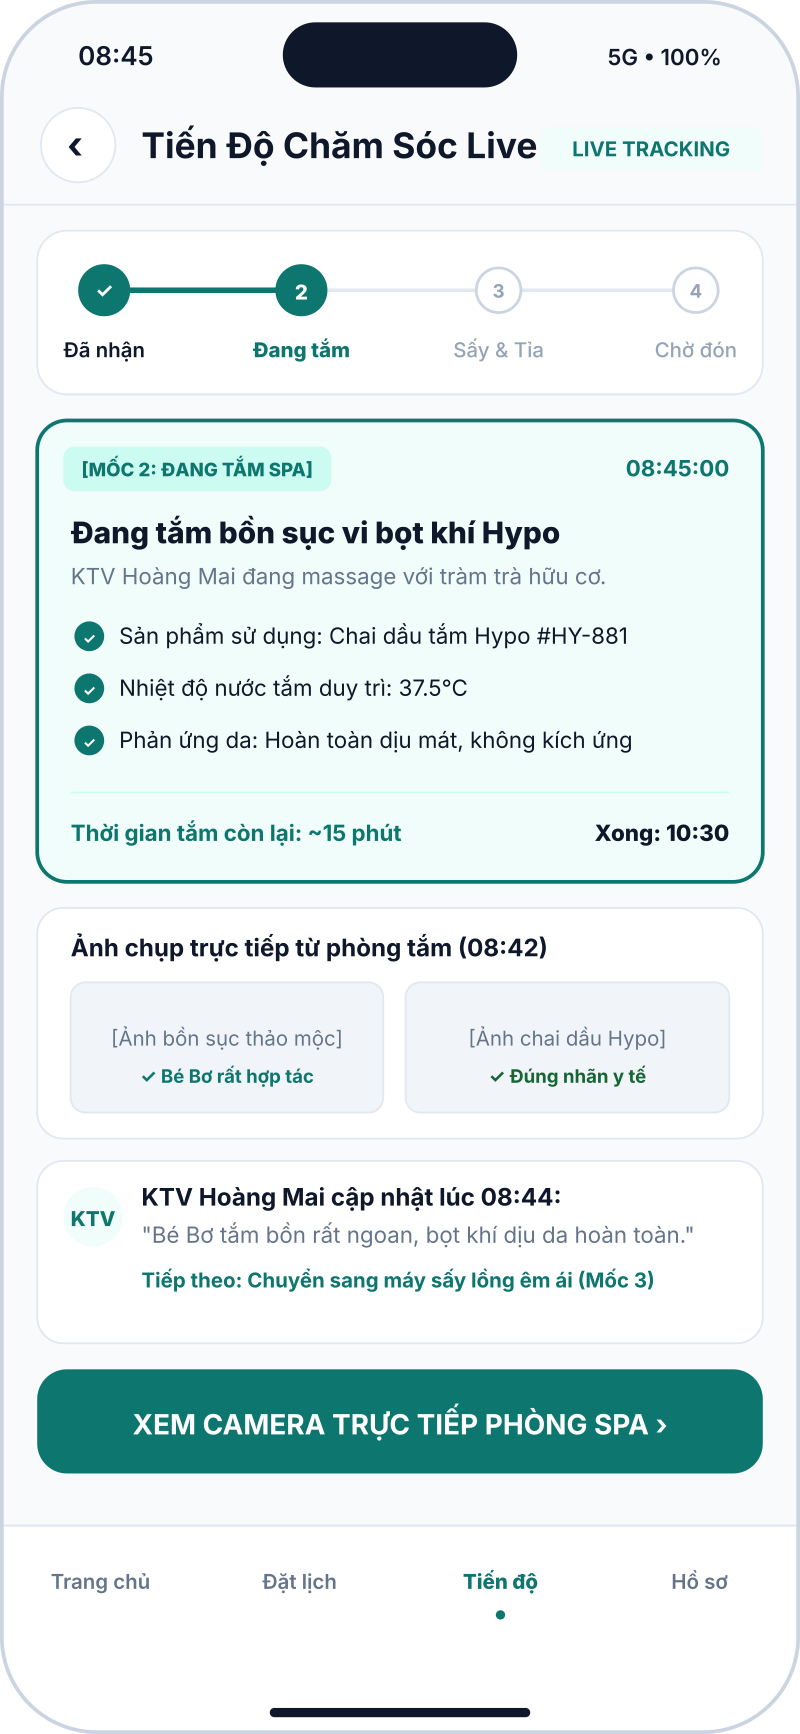
\includegraphics[height=4.4cm, keepaspectratio]{img/wf_15_tracking.png}\\[0.5mm]
          {\tiny \textbf{Live Tracking}}
        \end{column}
      \end{columns}
      \vspace{1mm}
      {\tiny \color{gray} Bộ 32 Wireframes vector SVG chuẩn iPhone 14 Pro Max ($430 \times 932\text{px}$)}
    \end{column}
  \end{columns}
\end{frame}


% Slide 7: Bản mẫu tương tác: 4 Trụ cột giải pháp số hóa
% Slide 7: Bản mẫu tương tác: 4 Trụ cột giải pháp số hóa
\begin{frame}{Bản Mẫu Tương Tác: 4 Trụ Cột Giải Pháp Số Hóa}
  \framesubtitle{\color{PetcareSecondary}\textbf{Hiện thực hóa trải nghiệm: 4 Trụ cột tương tác cao chuẩn Mobile-first}}

  \begin{columns}[T]
    % Cột 1: Đặt lịch tức thì
    \begin{column}{0.24\textwidth}
      \centering
      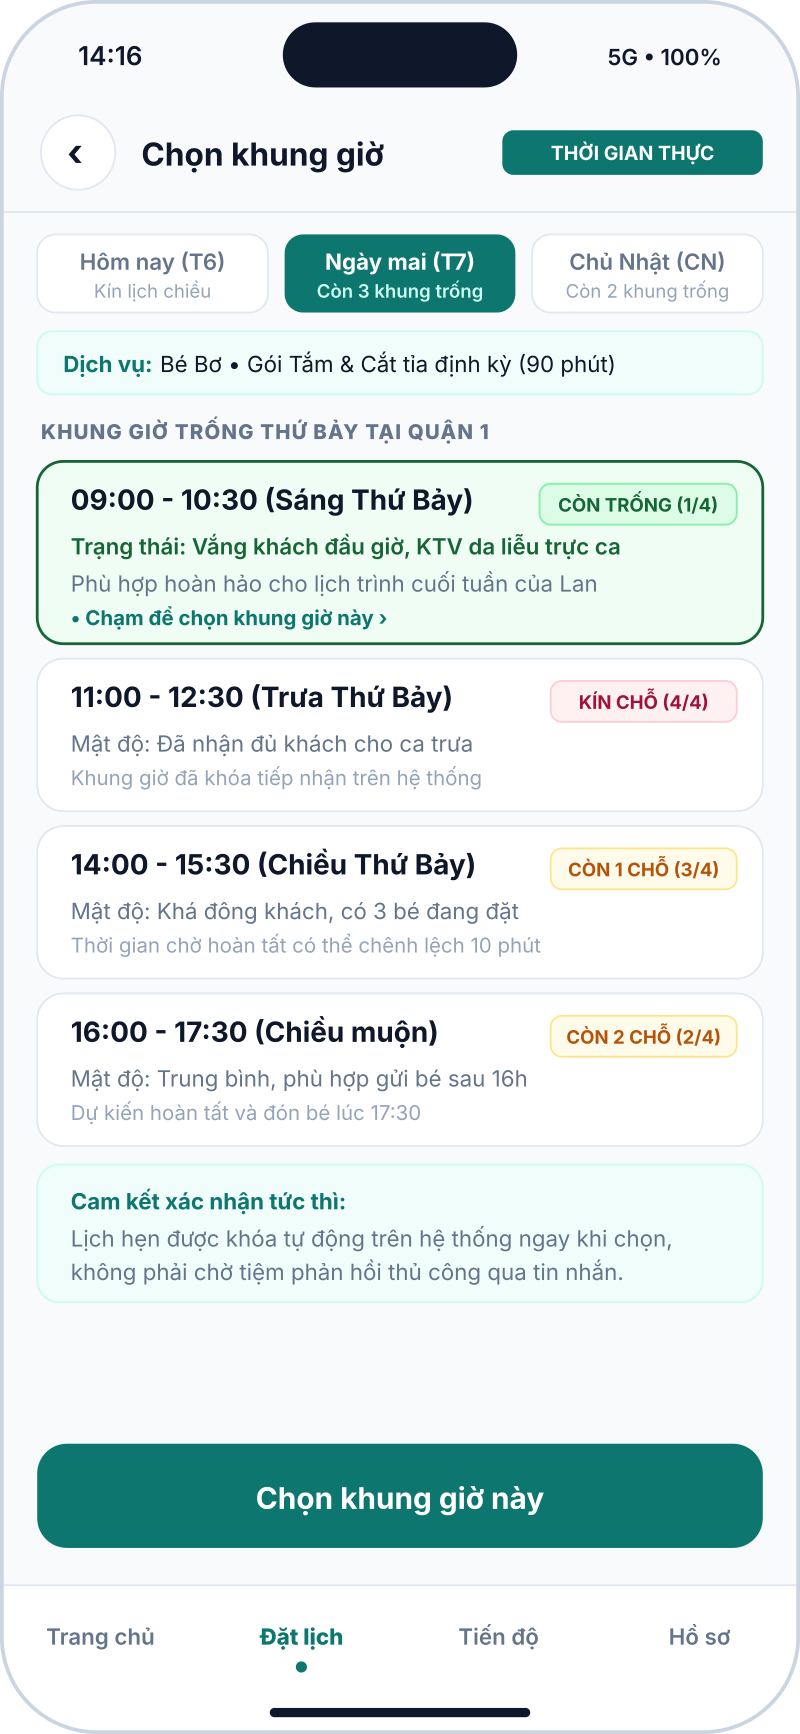
\includegraphics[height=4.1cm, keepaspectratio]{img/proto_p1_g1_02.png}\\[1mm]
      \begin{block}{\centering \tiny \textbf{1. Đặt lịch tức thì}}
        \tiny Khóa giờ trống real-time, cấp mã hẹn \& QR ngay lập tức ($<$ 40s).
      \end{block}
    \end{column}

    % Cột 2: Cảnh báo dị ứng đỏ
    \begin{column}{0.24\textwidth}
      \centering
      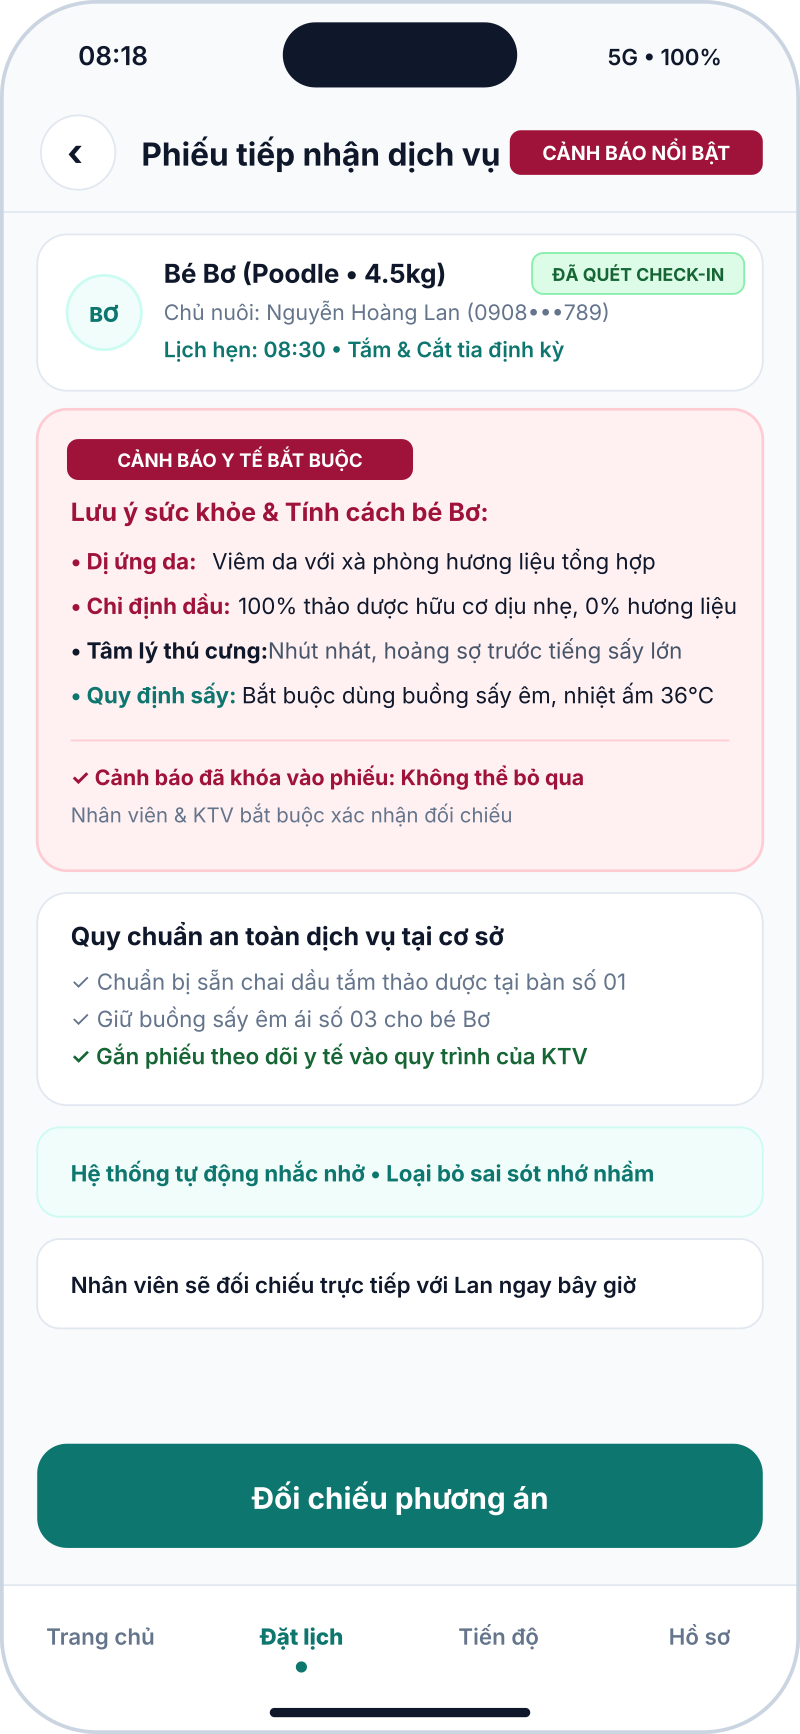
\includegraphics[height=4.1cm, keepaspectratio]{img/proto_p1_g2_03.png}\\[1mm]
      \begin{block}{\centering \tiny \textbf{2. Cảnh báo dị ứng}}
        \tiny Tự động gắn nhãn y tế đỏ; biên bản bàn giao an toàn 2 lớp tại tiệm.
      \end{block}
    \end{column}

    % Cột 3: Live Tracking 4 mốc
    \begin{column}{0.24\textwidth}
      \centering
      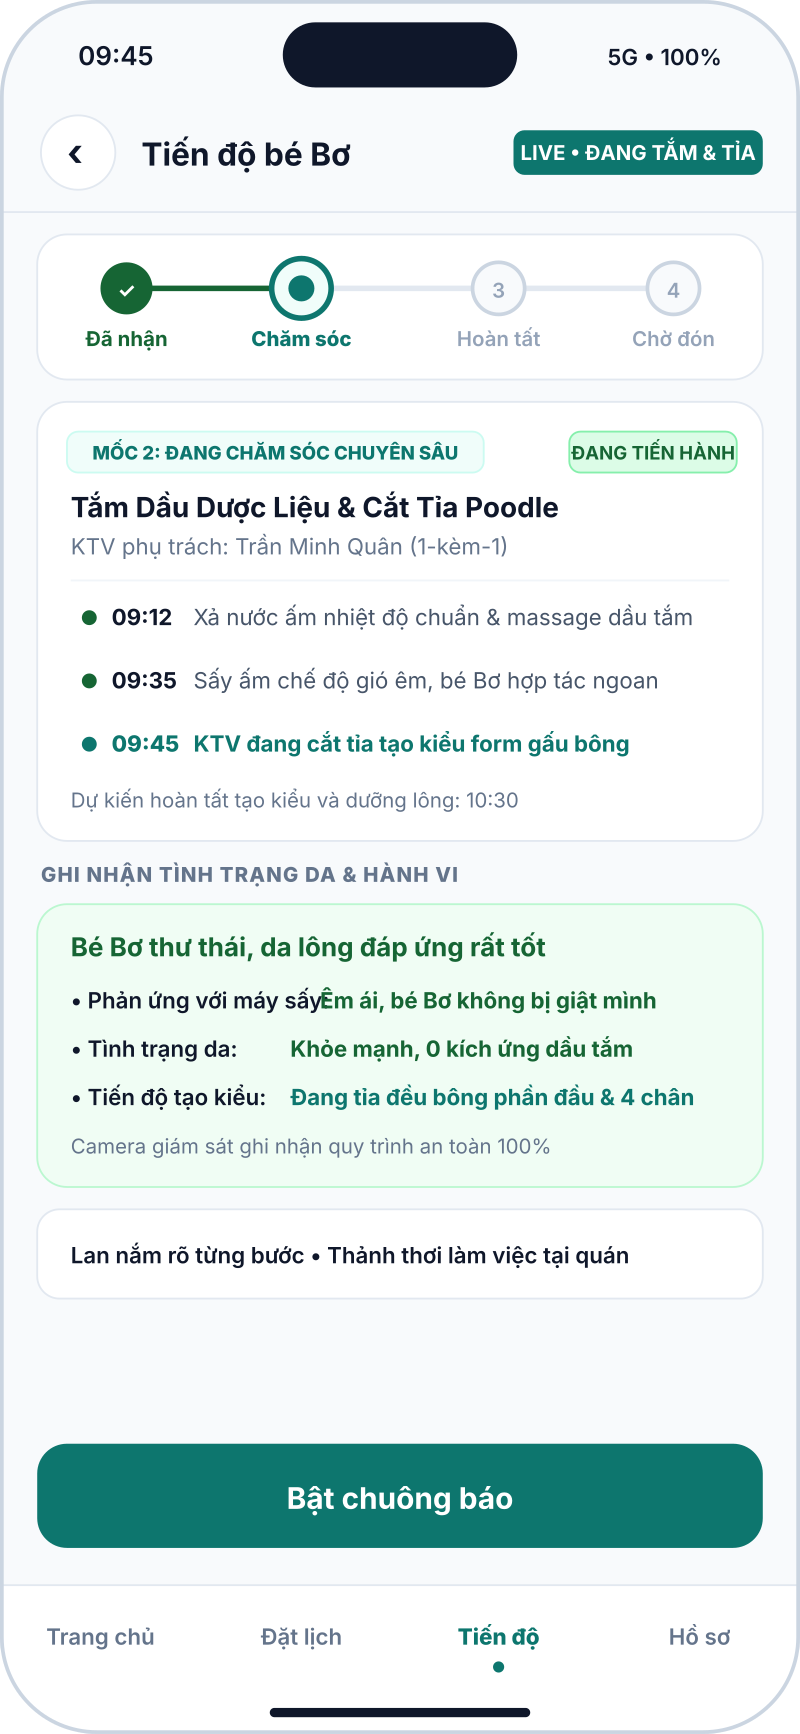
\includegraphics[height=4.1cm, keepaspectratio]{img/proto_p1_g3_02.png}\\[1mm]
      \begin{block}{\centering \tiny \textbf{3. Live Tracking 4 mốc}}
        \tiny Cập nhật từng phút qua 4 mốc chuẩn hóa kèm Push Notification.
      \end{block}
    \end{column}

    % Cột 4: Nhật ký & Rebook
    \begin{column}{0.24\textwidth}
      \centering
      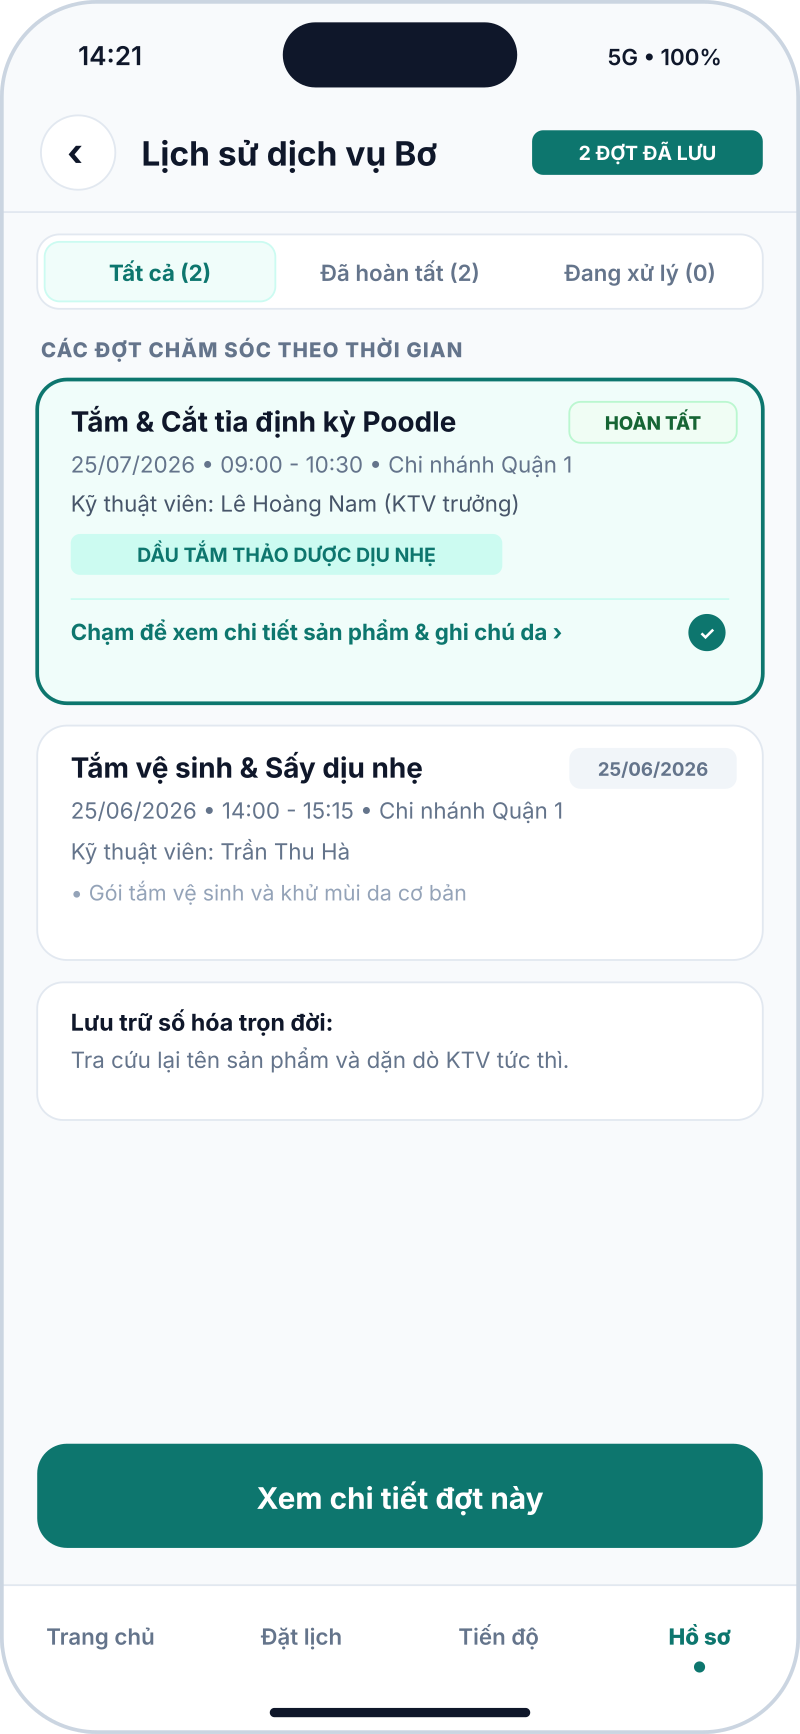
\includegraphics[height=4.1cm, keepaspectratio]{img/proto_p1_g4_02.png}\\[1mm]
      \begin{block}{\centering \tiny \textbf{4. Nhật ký \& Rebook}}
        \tiny Lưu trữ phác đồ dầu tắm, ảnh kiểm tra da lông \& đặt lại lịch 1 chạm.
      \end{block}
    \end{column}
  \end{columns}

  \vspace{1mm}
  \begin{center}
    \tiny \color{PetcareDark}
    \textbf{Độ trung thực cao (Hi-Fi Prototype):} 37 màn hình tương tác vector SVG chuẩn Figma kết hợp Web Runtime React + TypeScript.
  \end{center}
\end{frame}


% Slide 8: Đánh giá khả năng sử dụng: Dữ liệu SUS 84.5 & TSR 100%
% Slide 8: Đánh giá khả năng sử dụng: Dữ liệu SUS 84.5 & TSR 100%
\begin{frame}{Đánh Giá Khả Năng Sử Dụng: Chứng Thực Thực Nghiệm}
  \framesubtitle{\color{PetcareSecondary}\textbf{Chứng thực bằng số liệu: SUS đạt 84.5 điểm và tỷ lệ hoàn thành tác vụ 100\%}}

  % 4 Thẻ số liệu lớn hàng đầu
  \begin{columns}[c]
    \begin{column}{0.24\textwidth}
      \begin{block}{\centering \tiny \textbf{Thang đo SUS}}
        \centering \vspace{0.5mm}
        {\large \textbf{\color{PetcareSuccess}84.5 / 100}}\\[0.5mm]
        {\tiny \textbf{Grade A / Excellent}}
      \end{block}
    \end{column}
    \begin{column}{0.24\textwidth}
      \begin{block}{\centering \tiny \textbf{Tỷ lệ hoàn thành (TSR)}}
        \centering \vspace{0.5mm}
        {\large \textbf{\color{PetcareSuccess}100\% (5/5)}}\\[0.5mm]
        {\tiny Không cần trợ giúp}
      \end{block}
    \end{column}
    \begin{column}{0.24\textwidth}
      \begin{block}{\centering \tiny \textbf{Thời gian Đặt lịch (T1)}}
        \centering \vspace{0.5mm}
        {\large \textbf{\color{PetcarePrimary}39.0 giây}}\\[0.5mm]
        {\tiny \textbf{0 lỗi phát sinh}}
      \end{block}
    \end{column}
    \begin{column}{0.24\textwidth}
      \begin{block}{\centering \tiny \textbf{Tra cứu Tiến độ (T3)}}
        \centering \vspace{0.5mm}
        {\large \textbf{\color{PetcarePrimary}18.8 giây}}\\[0.5mm]
        {\tiny Nắm bắt ngay 1 chạm}
      \end{block}
    \end{column}
  \end{columns}

  \vspace{1.5mm}

  \begin{columns}[T]
    % Bảng đo lường 4 tác vụ
    \begin{column}{0.62\textwidth}
      \begin{table}
        \centering
        \tiny
        \renewcommand{\arraystretch}{1.15}
        \begin{tabularx}{\textwidth}{|l|c|c|c|X|}
          \hline
          \rowcolor{PetcarePrimary!15}
          \textbf{Tác vụ kiểm thử} & \textbf{TSR} & \textbf{TG TB} & \textbf{Lỗi} & \textbf{Phản hồi người dùng} \\ \hline
          \textbf{T1: Đặt lịch \& nhận mã} & 100\% & 39.0s & 0 & Ma trận trực quan, thao tác cực nhanh. \\ \hline
          \textbf{T2: Dặn dò y tế \& dị ứng} & 100\% & 57.4s & 5 & Ô ghi chú ban đầu bị ẩn sâu trong menu. \\ \hline
          \textbf{T3: Live Tracking 4 mốc} & 100\% & 18.8s & 1 & Thanh tiến trình rõ ràng, rất an tâm. \\ \hline
          \textbf{T4: Tra cứu lịch sử \& Rebook} & 100\% & 30.8s & 0 & Xem nhanh tên dầu tắm, đặt lại mượt mà. \\ \hline
        \end{tabularx}
      \end{table}
    \end{column}

    % Cột nhận xét định tính
    \begin{column}{0.36\textwidth}
      \begin{exampleblock}{\scriptsize \textbf{Nhận định từ chuyên gia \& Người dùng}}
        \tiny
        $\bullet$ \textbf{Điểm mạnh vượt bậc:} Tốc độ đặt lịch tức thì và tính minh bạch của Live Tracking giải tỏa triệt để áp lực tâm lý.\\
        $\bullet$ \textbf{Điểm nghẽn cần tối ưu:} Vị trí nhập dặn dò y tế (T2) cần được đưa thẳng ra form đặt lịch chính để tránh mất thời gian tìm kiếm.
      \end{exampleblock}
    \end{column}
  \end{columns}
\end{frame}


% Slide 9: Thiết kế cuối cùng: 4 Cải tiến then chốt sau kiểm thử
% Slide 9: Thiết kế cuối cùng: 4 Cải tiến then chốt sau kiểm thử
\begin{frame}{Thiết Kế Cuối Cùng: Tinh Chỉnh Sau Đánh Giá}
  \framesubtitle{\color{PetcareSecondary}\textbf{Tối ưu hóa liên tục: 4 Cải tiến then chốt từ phản hồi thực nghiệm}}

  \begin{columns}[T]
    % Cột 1: 4 Cải tiến cụ thể
    \begin{column}{0.54\textwidth}
      \begin{itemize}
        \setlength\itemsep{1.5mm}
        \footnotesize
        \item \textbf{1. Đưa thẻ Dặn dò y tế thẳng vào Form Đặt lịch:} Khắc phục 5 lỗi tìm kiếm ở T2; hệ thống tự nạp dị ứng đã lưu và cho phép sửa nhanh tại chỗ.
        \item \textbf{2. Tăng tương phản Ma trận thời gian:} Viền xanh đậm \texttt{\#0D9488} cho giờ khả dụng; xám mờ \texttt{\#D1D5DB} kèm nhãn ``Hết chỗ'' rõ nét.
        \item \textbf{3. Nâng cấp biểu tượng 4 mốc tiến độ:} Mốc 2 thêm hiệu ứng kéo spa; Mốc 3 dấu tích xanh hoàn tất; Mốc 4 chuông gọi đón trực quan.
        \item \textbf{4. Tối ưu phân hệ Lịch sử \& Hóa đơn:} Hiển thị ca mới nhất ở đầu danh sách, kèm nút xem chi tiết phác đồ dầu tắm và Rebook 1 chạm.
      \end{itemize}
    \end{column}

    % Cột 2: Bảng đối sánh Before & After
    \begin{column}{0.44\textwidth}
      \begin{table}
        \centering
        \tiny
        \renewcommand{\arraystretch}{1.2}
        \begin{tabularx}{\textwidth}{|l|X|X|}
          \hline
          \rowcolor{PetcarePrimary!15}
          \textbf{Hạng mục} & \textbf{Trước kiểm thử} & \textbf{Sau cải tiến} \\ \hline
          \textbf{Dặn dò dị ứng} & Nằm sâu trong menu Hồ sơ (5 lỗi). & Nằm ngay form Đặt lịch (\textbf{0 lỗi}). \\ \hline
          \textbf{Ma trận giờ} & Màu sắc nhạt trên màn hình tối. & Tương phản cao, nhãn ``Hết chỗ''. \\ \hline
          \textbf{Live Tracking} & 4 nút mốc tĩnh, màu đồng nhất. & Biểu tượng động \& phân biệt màu. \\ \hline
          \textbf{Lịch sử DV} & Danh sách phẳng, không phân loại. & Ưu tiên ca gần nhất \& Rebook 1 chạm. \\ \hline
        \end{tabularx}
      \end{table}

      \vspace{0.5mm}
      \begin{center}
        \scriptsize \color{PetcareSuccess}
        \textbf{Kết quả:} Rút ngắn thời gian tác vụ T2 từ 57.4s xuống $<$ 35s.
      \end{center}
    \end{column}
  \end{columns}

  \vspace{1.5mm}
  \begin{block}{\centering \scriptsize \textbf{Triết lý hoàn thiện}}
    \centering \tiny
    Lắng nghe tiếng nói người dùng thực tế $\rightarrow$ Loại bỏ ma sát tương tác $\rightarrow$ Đạt chuẩn trải nghiệm \textbf{Zero Friction UX}.
  \end{block}
\end{frame}


% Slide 10: Tầm nhìn tương lai, Đóng góp & Hạn chế
% Slide 10: Tầm nhìn tương lai, Đóng góp & Hạn chế
\begin{frame}{Tầm Nhìn Tương Lai \& Đóng Góp Thực Tiễn}
  \framesubtitle{\color{PetcareSecondary}\textbf{Khẳng định giá trị: Đóng góp thực tiễn \& Lộ trình mở rộng nền tảng tương lai}}

  \begin{columns}[T]
    % Cột 1: 3 Đóng góp thực tiễn của đề tài
    \begin{column}{0.48\textwidth}
      \begin{block}{\footnotesize \textbf{3 Đóng góp cốt lõi của đề tài}}
        \scriptsize
        \begin{itemize}
          \setlength\itemsep{1mm}
          \item \textbf{Phương pháp luận UCD chuẩn mực:} Bộ artifact hoàn chỉnh: 2 Persona, 2 Value Maps, 6 Storyboards, 32 Wireframes và 37 màn hình Prototype.
          \item \textbf{Giá trị thực tiễn vượt trội:} Cắt giảm thời gian đặt lịch xuống $<$ 40s; triệt tiêu 100\% rủi ro quên dị ứng; minh bạch hóa toàn bộ 4 mốc tiến độ.
          \item \textbf{Sản phẩm phần mềm hoàn chỉnh:} Web App React + TypeScript tương tác mượt mà, vượt qua \textbf{39/39 kịch bản test tự động}, đạt SUS \textbf{84.5/100}.
        \end{itemize}
      \end{block}
    \end{column}

    % Cột 2: Hạn chế & 4 Lộ trình mở rộng tương lai
    \begin{column}{0.48\textwidth}
      \begin{exampleblock}{\footnotesize \textbf{Lộ trình phát triển tương lai}}
        \scriptsize
        \begin{itemize}
          \setlength\itemsep{1mm}
          \item \textbf{Staff App chuyên biệt:} Ứng dụng di động cho kỹ thuật viên quét QR đổi mốc và chụp ảnh kiểm tra da lông.
          \item \textbf{Real-time Backend (WebSocket):} Gửi thông báo đẩy Native Push qua APNs/FCM tức thời giữa nhiều thiết bị.
          \item \textbf{Trợ lý ảo AI (AI Care):} Phân tích giống loài và tiền sử để gợi ý chu kỳ spa, nhắc lịch tiêm phòng thông minh.
          \item \textbf{Mở rộng hệ sinh thái:} Tích hợp dịch vụ đưa đón thú cưng (\textit{Pet Taxi}) và cổng thanh toán trực tuyến bảo mật.
        \end{itemize}
      \end{exampleblock}
    \end{column}
  \end{columns}

  \vspace{1mm}
  \begin{center}
    \scriptsize \color{gray}
    \textit{Hạn chế khách quan: Quy mô mẫu khảo sát 6 người và kiểm thử 5 người trong phạm vi môn học; dữ liệu thời gian thực hiện mô phỏng phía Client.}
  \end{center}
\end{frame}


% Slide 11: Lời cảm ơn & Phiên thảo luận Q&A
% Slide 11: Lời cảm ơn & Phiên thảo luận Q&A
\begin{frame}{Phiên Thảo Luận \& Hỏi Đáp (Q\&A)}
  \framesubtitle{\color{PetcareSecondary}\textbf{Chân thành cảm ơn Quý Thầy Cô và Hội đồng đã chú ý lắng nghe!}}

  \vspace{2mm}

  \begin{center}
    {\large \bfseries \color{PetcarePrimary} HỆ THỐNG HỖ TRỢ ĐẶT LỊCH, GỬI YÊU CẦU\\VÀ THEO DÕI QUÁ TRÌNH CHĂM SÓC THÚ CƯNG}\\[3mm]
    {\footnotesize \color{PetcareDark}\textit{``Công nghệ vị nhân sinh -- Nâng tầm trải nghiệm chăm sóc thú cưng an toàn, minh bạch và hạnh phúc.''}}
  \end{center}

  \vspace{3mm}

  \begin{columns}[c]
    \begin{column}{0.46\textwidth}
      \begin{block}{\footnotesize \textbf{Lời tri ân sâu sắc}}
        \scriptsize
        Nhóm xin chân thành cảm ơn:\\[1mm]
        $\bullet$ \textbf{Lê Thị Nhàn}\\
        $\bullet$ \textbf{Lương Vĩ Minh}\\[1mm]
        đã tận tình hướng dẫn, định hướng phương pháp luận HCI và góp ý chuyên sâu trong suốt quá trình thực hiện đề tài.
      \end{block}
    \end{column}

    \begin{column}{0.48\textwidth}
      \begin{exampleblock}{\footnotesize \textbf{Phiên thảo luận \& Đóng góp ý kiến}}
        \scriptsize
        \textbf{Nhóm sinh viên thực hiện (Nhóm 10):}\\[1mm]
        $\bullet$ \textbf{23127327} -- Lưu Ngô Quốc Bảo\\
        $\bullet$ \textbf{23127328} -- Nguyễn Quốc Bảo\\
        $\bullet$ \textbf{23127498} -- Nguyễn Trọng Tín\\[2mm]
        \centering
        {\normalsize \bfseries \color{PetcareSecondary} XIN MỜI QUÝ THẦY CÔ ĐẶT CÂU HỎI}
      \end{exampleblock}
    \end{column}
  \end{columns}
\end{frame}


\end{document}
